\documentclass[12pt]{article}
\usepackage[top=0.5in, bottom=0.5in]{geometry}
\usepackage{amsmath}
\usepackage{mathtools}
\usepackage{amssymb}
\usepackage{pifont}
\usepackage{tikz-qtree}
\usepackage{tikz}
\usetikzlibrary{trees}
\usepackage{hyperref}

\newcommand{\cmark}{\ding{51}}%
\newcommand{\xmark}{\ding{55}}%
\newcommand\tab[1][1cm]{\hspace*{#1}}

\begin{document}

\title{Course Project - Assignment}
\author{Austin Bennett}
\maketitle

\section{Data Collection}

\tab The data used for this assignment was retrieved from The Cancer Imaging Archive (TCIA). The dataset used was 
\href{https://wiki.cancerimagingarchive.net/pages/viewpage.action?pageId=61080958}{A Single-cell Morphological Dataset of Leukocytes from AML Patients and Non-malignant Controls (AML-Cytomorphology-LMU)}. \\ \\
\tab "The Munich AML Morphology Dataset contains 18,365 expert-labeled single-cell images taken from peripheral blood smears of 100 patients diagnosed with Acute Myeloid Leukemia at Munich University Hospital between 2014 and 2017, as well as 100 patients without signs of hematological malignancy. Image acquisition was done using a M8 digital microscope / scanner (Precipoint GmbH, Freising, Germany) at 100-fold optical magnification and oil immersion. Pathological and non-pathological leukocytes were classified into a standard morphological classification scheme derived from clinical practice by trained experts. To quantify inter- and intra-rater variability of examiners, a subset of images was re-annotated up to two times. The dataset has been used by the authors to train a convolutional neural network for single-cell morphology classification." ~\cite{Matek}







\section{Data Format Description}
\tab The dataset contains 18,365 .tiff (Tagged Image File Format) files at 626 kilabytes per image we total up to approximately 11 gigabytes worth of images. The dataset also includes a txt file that contains the abbreviations and their respective full names for all 15 morphological types covered in this research. Lastly there is a .dat annotation file that consists of 4 columns of data: the name of the respective image file, the morphological class assigned during the gold-standard annotation, if the image was chosen for re-annotation there will be another annotation else nan, finally if the image was chosen for re-annotation it will be annotated again 11 months after the first re-annotation. All columns were listed in respective order.

\newpage






\section{Descriptive Statistics}
\tab Since the dataset consists purely of thousands of images, i will provide a graph showing the distribution of our 15 morphological classes within the dataset.
As noted in the Data Format Description, there are randomly selected 

\begin{figure}[!htb]
		\centering
		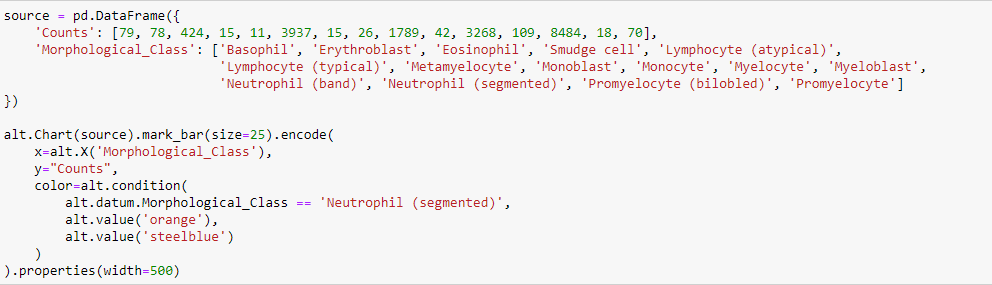
\includegraphics[width=1\textwidth]{part3_code.png}
		\caption{\label{: }Altair code for morphological class distribution}
	\end{figure} 
\begin{figure}[!htb]
		\centering
		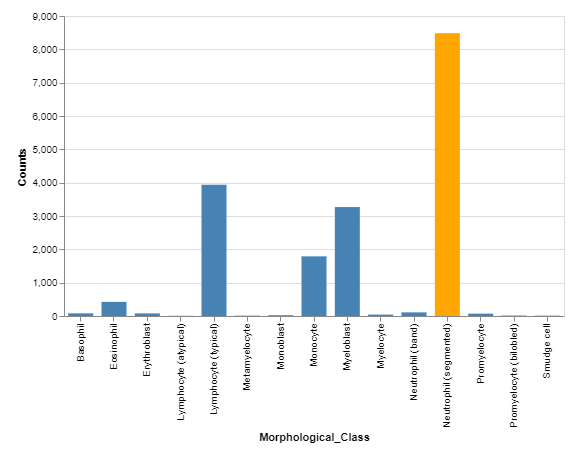
\includegraphics[width=1\textwidth]{part3_image.png}
		\caption{\label{: }Altair plot for morphological class distribution}
	\end{figure}






\newpage

\section{Data Analysis, Visualization, and Insights}
\tab As described in Data Format Description, random images in the dataset were selected for re-annotation after a brief lull. These re-annotated images are denoted in the annotation file and are important because although most of them were confirmed to be their original guess, some initial guesses were contradicted in their re-annotation.

\begin{figure}[!htb]
		\centering
		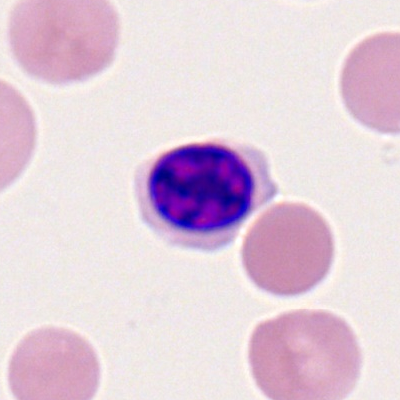
\includegraphics[width=0.4\textwidth]{EBO_0033.png}
		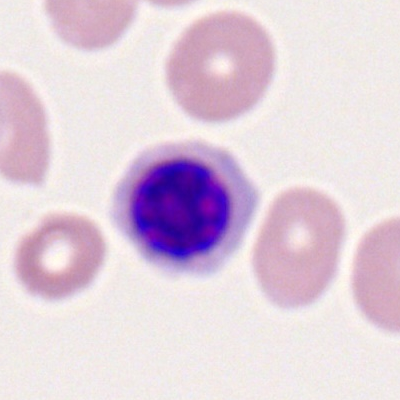
\includegraphics[width=0.4\textwidth]{EBO_0039.png}
		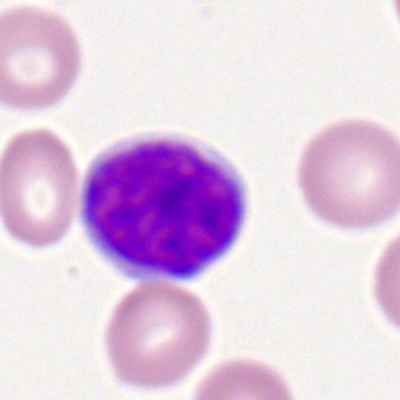
\includegraphics[width=0.4\textwidth]{LYT_0787.png}
		\caption{\label{: }Example images of erythoblasts and lymphocytes (typical)}
	\end{figure} 

\tab The top-left image in Figure 3 is an example of a leukocyte that was originally classified as an erythoblast but was re-annotated on both attempts as a lymphocyte (typical). The top-right image in Figure 3 is an example of a leukocyte that was originally classified as an erythoblast and was reconfirmed on both re-annotations. And finally the bottom image is an example of a leukocyte originally classified as a lymphocyte (typical) and was reconfirmed on both re-annotations.\\
\tab To the eye of someone without expertise in this particular field the differences between these leukocytes is impossible to distinguish. As I am not someone with particular expertise on leukocytes, for simplicty I will use the data of all the original annotations of each leukocyte for the image classifier. \\
\newpage
\tab It is also important to note that from the Descriptive Statistics section, we can clearly tell that there is only a substantial amount of training data for 4 types of leukocytes:  lymphocytes (typical), monocytes, myeloblasts, and neutrophils (segmented). With such a small amount of training data for our other 11 morphological types, a simple machine learning algorithm will not do. A more complex algorithm will be necessary to accurately predict our leukocytes. We will employ a convolutional neural network to aide us with accurately classifying the leukocytes into their morphological classes.

\begin{figure}[!htb]
		\centering
		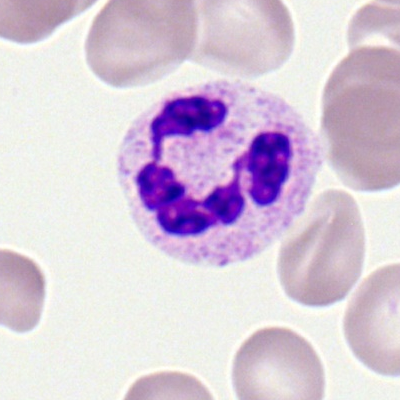
\includegraphics[width=0.4\textwidth]{NGS_0086.png}
		\caption{\label{: }Neurophil (segmented) \#86, the most commonly appearing leukocyte in the dataset}
	\end{figure} 


\section{Future Plans}
\tab Unfortunately for me, even though the dataset consists of 100 patients with and without signs of hematological malignancy and 100 patients, which cells belonged to each group were not recorded. I was very interested in being able to see if our convolutional neural network would be able to detect some pattern of hematological malignancy as well as morphological classifcation. Since that data is not recorded in the dataset though, I will stick to the basic morphological classifcation. First, I plan on using a built in python library to construct the initial neural network. After obtaining a baseline, I will see how far I can take the accuracy and if there is still significant room for improvement I may try to indulge in a newer take on image classification called\href{https://arxiv.org/pdf/1710.09829.pdf}{capsule networks}. If the convolutional neural network fails to provide incredible accuracy for our morphological classifcation, it should be interesting to explore the concept of capsule networks. Geoffrey E. Hinton's article outlines a significant amount of the concept of capsule networks and should be enough in conjunction with more recent work on capsule networks to try and deploy it.


\newpage
\section{Results and Conclusion}
\tab I learned some interesting things from my endeavors in applying a Convultional Neural Network algorithm to this dataset. Among the interesting things were quite a few overlooked obstacles. One of the obstacles was the size of the dataset which I did not realize until actually trying to perform some machine learning on the dataset. Due to the size of the dataset I had to develop a way to send batches of the file into the training algorithm separately and then combine the results. Another issue that I encountered was how long the machine learning actually took to perform on a large dataset like this. Due to my own time constraints I was forced to use a fairly weak model architecture for my CNN algorithm to save time, making each training epoch take about 3 hours. Using a more proper model architecture for this dataset would have taken my computer approximately 36 hours per training epoch. As such the results suffered fairly significantly, only producing a final validation accuracy of 73.08\% after 3 epochs.
\begin{figure}[!htb]
		\centering
		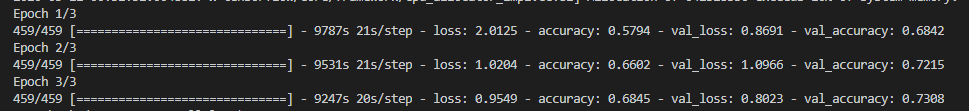
\includegraphics[width=0.9\textwidth]{ml_results.png}
		\caption{\label{: } Convolutional Neural Network results}
	\end{figure} 

Even though this algorithm was not able to produce sufficiently accurate classification results, there is no doubt in my mind that a proper model architecture would have been able to get the accuracy up to 90\% or above within 5 epochs. Another thing to note is that this dataset had 15 total classifiers, while 99\% of the dataset was for only 3 of the classifiers which likely led to some confusion for the algorithm. When the weak model architecture was tested for a binary classifier adaptation of the model it produced extremely high accuracy: 99\% or above within 3 epochs.

\begin{figure}[!htb]
		\centering
		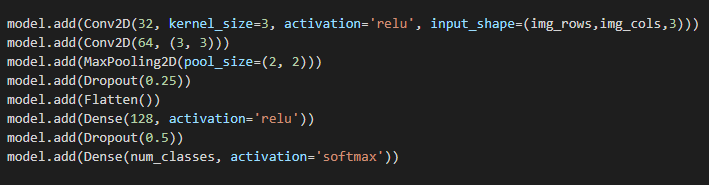
\includegraphics[width=0.9\textwidth]{weak_architecture.png}
		\caption{\label{: } Example of the weak model architecture used}
	\end{figure} 




\newpage
\section{Acknowledgements}
The following python libraries were used: \\
import matplotlib.pyplot as plt \\ 
import keras \\
from keras.utils import to\_categorical \\
from keras.models import Sequential \\
from keras.layers import Dense, Conv2D, Flatten, BatchNormalization, MaxPooling2D, Dropout \\ 
import os \\
from sklearn.model\_selection import train\_test\_split \\
import pandas as pd \\
from PIL import Image \\
import cv2 \\ 
import glob \\ 
import numpy as np \\
from skimage.io import imread \\
from skimage.transform import resize \\







\newpage
\bibliographystyle{plain}
\bibliography{mybib}






\end{document}